\documentclass[11pt]{article}


\usepackage{amsfonts}
\usepackage{fancyvrb}
\usepackage{url}
\usepackage{graphicx}
\usepackage{caption}
\usepackage{subcaption}

\setlength{\oddsidemargin}{0in}
\setlength{\evensidemargin}{0in}
\setlength{\textwidth}{6.5in}
\setlength{\topmargin}{0in}
\setlength{\headsep}{0.5in}
\setlength{\textheight}{8.5in}
\setcounter{page}{1}
%\pagestyle{empty}
%\hbadness=10000

\begin{document}
\huge
\noindent
{Discrete Optimization Assignment:}
\vspace{0.25cm}

\noindent
{\bf Graph Coloring}
\normalsize


\section{Problem Statement}

In this assignment you will design an algorithm to find the smallest {\em coloring} of a graph.\footnote{See \url{http://mathworld.wolfram.com/ChromaticNumber.html}}  You are provided with a graph and your task is to label the graph's nodes with as few colors as possible such that all pairs of nodes joined by an edge do not have the same color.  Figure \ref{fig:graph} illustrates a graph and a three coloring of that graph.  The nodes of the graph are labeled with black numbers while the coloring of the graph is labeled with white numbers.  You may notice that a three coloring is not a minimal coloring of this graph.  In fact, a two coloring is possible.

\begin{figure}[h]
        \centering
        \begin{subfigure}[b]{8.0cm}%{0.3\textwidth}
                \centering
                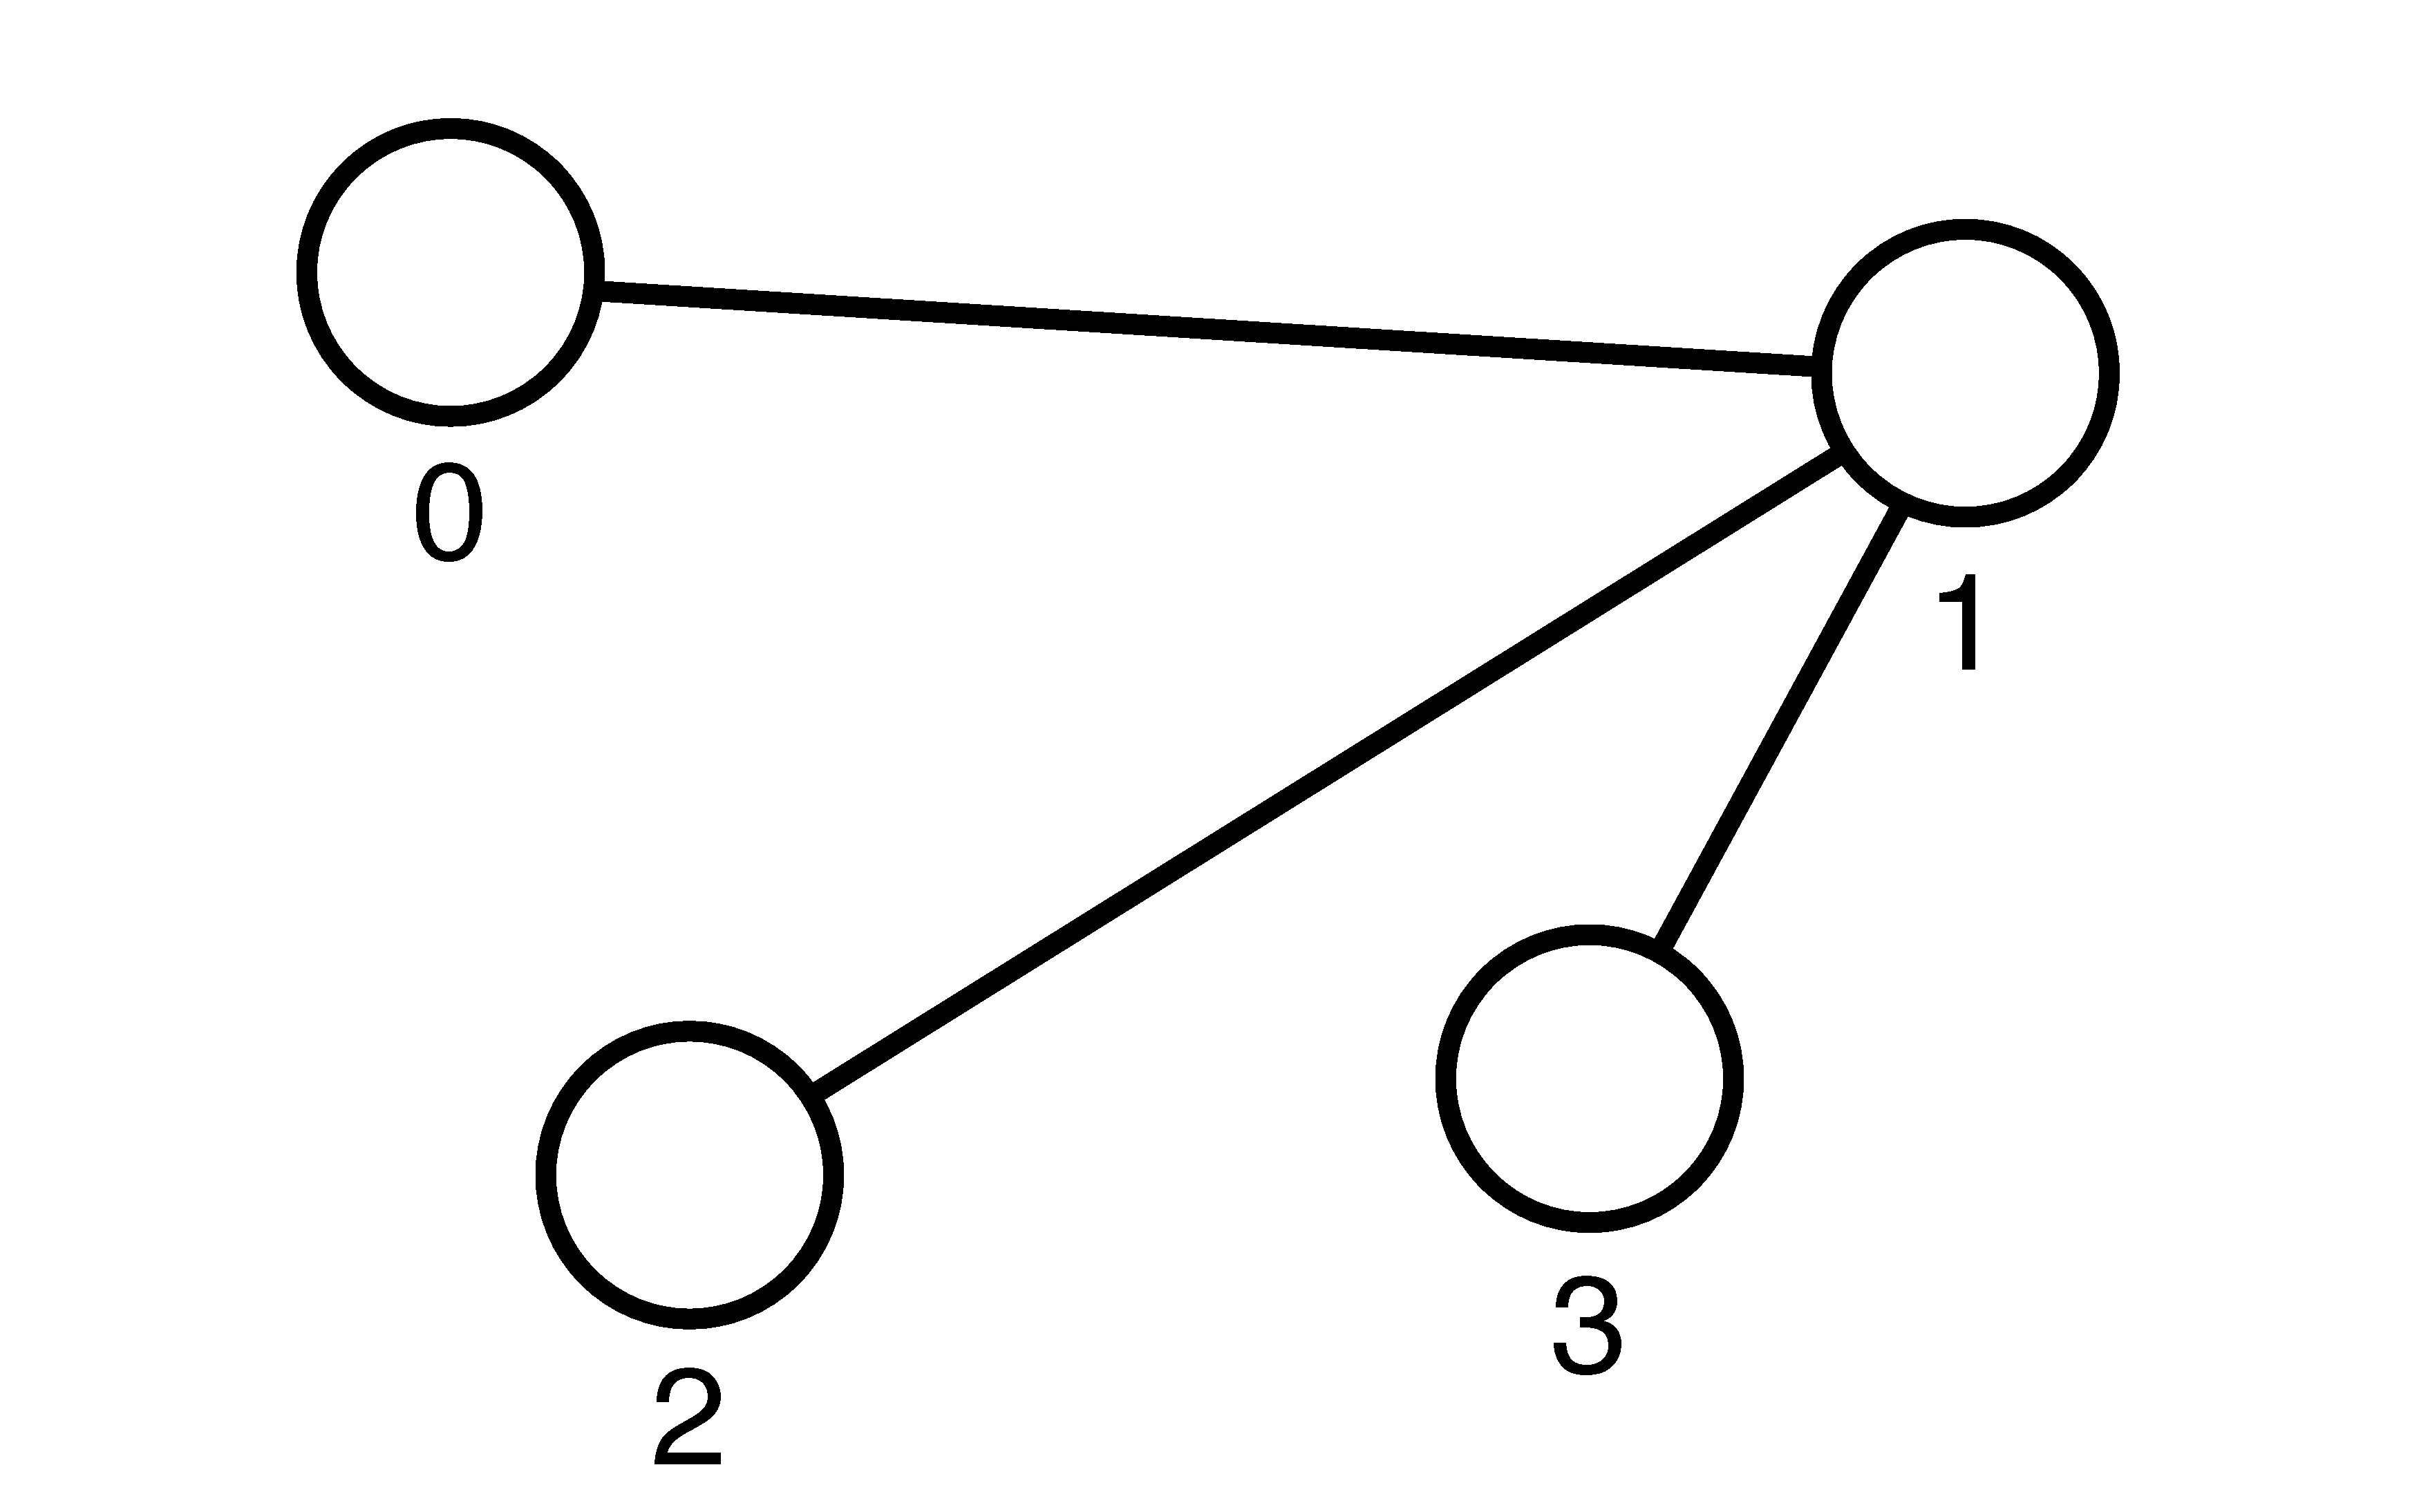
\includegraphics[width=8cm]{figures/coloring_1.pdf}
                \caption{A graph.}
                \label{fig:graph:input}
        \end{subfigure}%
        ~ %add desired spacing between images, e. g. ~, \quad, \qquad etc.
          %(or a blank line to force the subfigure onto a new line)
        \begin{subfigure}[b]{8.0cm}
                \centering
                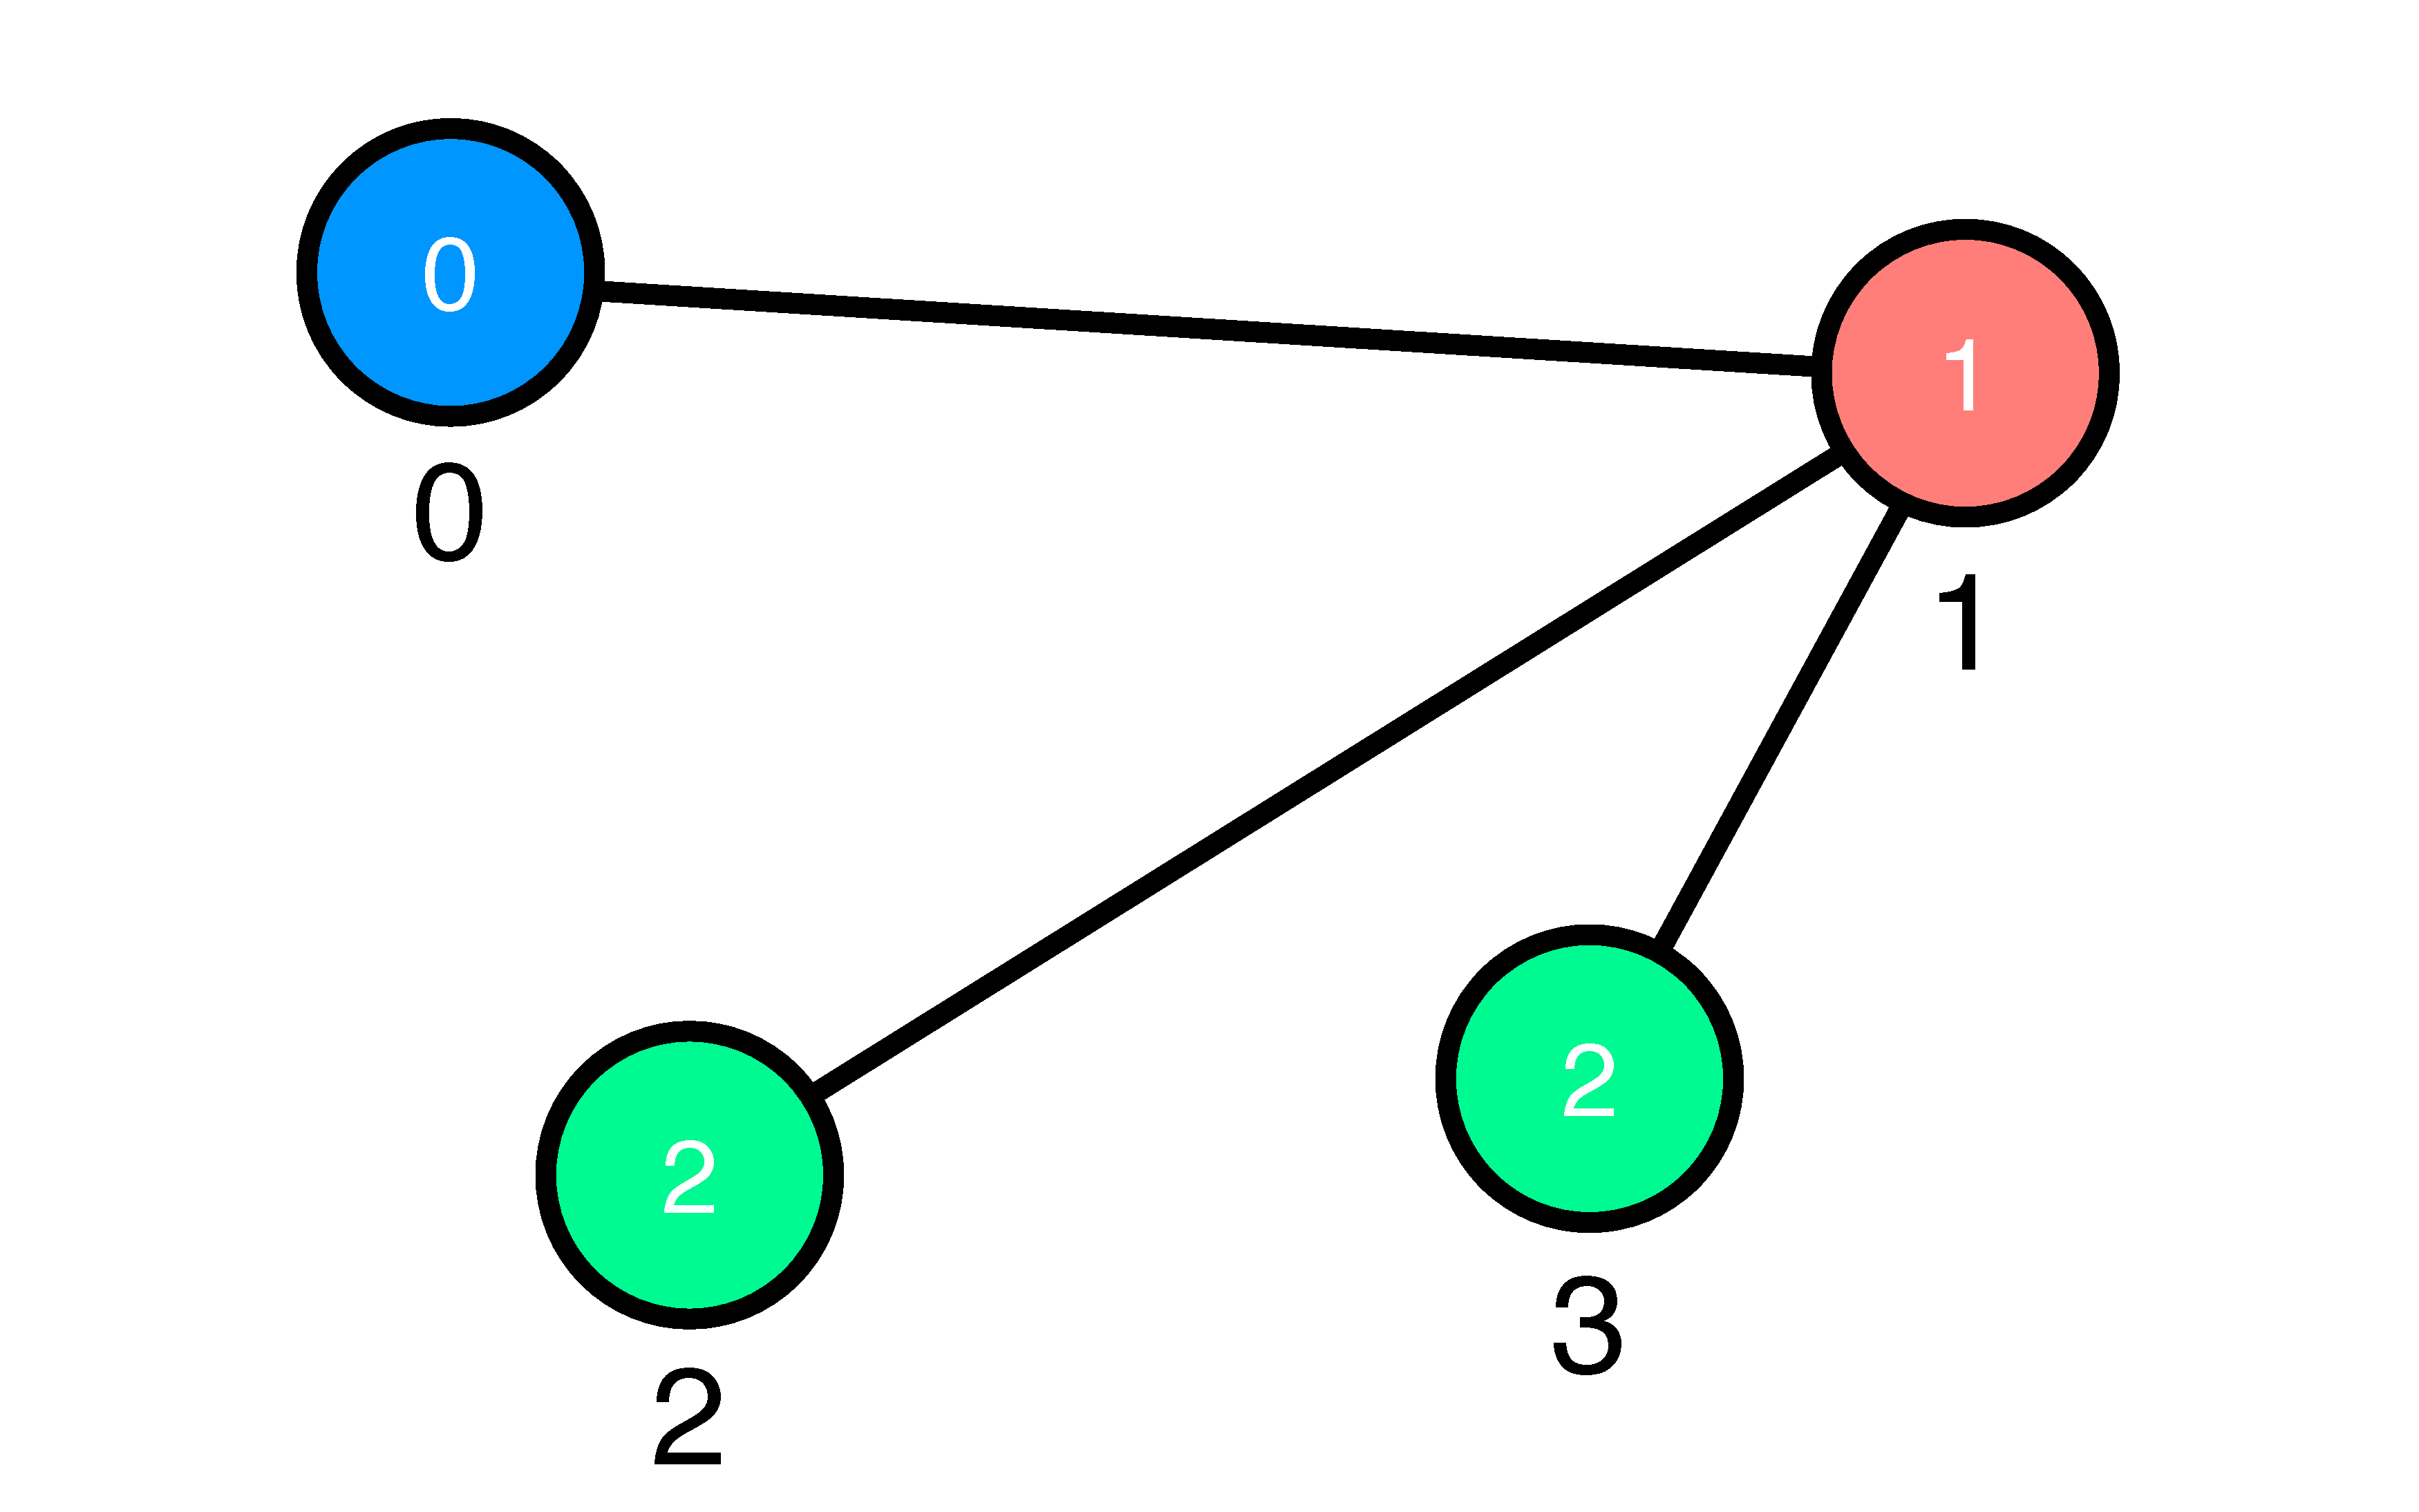
\includegraphics[width=8cm]{figures/coloring_2.pdf}
                \caption{A three-coloring of the graph.}
                \label{fig:graph:coloring}
        \end{subfigure}
        \caption{A Graph Coloring Example}\label{fig:graph}
\end{figure}

\section{Assignment}

Write an algorithm to minimize the coloring of a graph.  The problem is mathematically formulated in the following way.  Given a graph $G = \langle N, E \rangle$ with nodes $N = 0 \ldots n-1$ and edges $E$, let $c_i \in \mathbb{N}$ be a variable denoting the color of node $i$.  Then the graph coloring problem is formalized as the following optimization problem,
$$
\begin{array}{ll}
\mbox{minimize:} & \displaystyle \max_{i \in 0 \ldots n-1} c_i \\
\mbox{subject to:} & \\
     & c_i \neq c_j  \;\;\; (\langle i,j \rangle \in E)
\end{array}
$$

\section{Data Format Specification}

The input consists of $|E| + 1$ lines.  The first line contains two numbers $|N|$ and $|E|$.
It is followed by $|E|$ lines, each line represents an edge $\langle u_i, v_j \rangle$ where $u_i, v_j \in 0 \ldots |N|-1$.

\vspace{0.2cm}
\noindent
Input Format
\vspace{-0.2cm}
\begin{Verbatim}[frame=single]
|N| |E|
u_0 v_0
u_1 v_1
...
u_|E|-1 v_|E|-1
\end{Verbatim}
%
The output has two lines.  The first line contains two values $obj$ and $opt$.  $obj$ is the numbers of colors used in the coloring (i.e. the objective value).  $opt$ should be $1$ if your algorithm proved optimality and $0$ otherwise.  The next line is a list of $n$ values in $\mathbb{N}$, one for each of the $c_i$ variables.  This line encodes the solution.

\vspace{0.2cm}
\noindent
Output Format
\vspace{-0.2cm}
\begin{Verbatim}[frame=single]
obj opt
c_0 c_1 c_2 ... c_n-1
\end{Verbatim}
%
%It is essential that the value order in the solution output matches the value order of the input.  Otherwise the grader will misinterpret the output.

\paragraph{Examples} \mbox{}
%\vspace{0.1cm}
\noindent
(based on Figure \ref{fig:graph})

\vspace{0.2cm}
\noindent
Input Example
\vspace{-0.2cm}
\begin{Verbatim}[frame=single]
4 3
0 1
1 2
1 3
\end{Verbatim}

\vspace{0.2cm}
\noindent
Output Example
\vspace{-0.2cm}
\begin{Verbatim}[frame=single]
3 0
0 1 2 2
\end{Verbatim}

\section{Instructions}

Edit \texttt{solver.py} and modify the \texttt{solve\_it(input\_data)} function to solve the optimization problem described above.  The function argument, \texttt{input\_data}, contains the problem data in the format described above.  The return value of \texttt{solve\_it} is a solution to the problem in the output format described above.  Your \texttt{solve\_it} implementation can be tested with the command, 
\[ 
\texttt{python ./solver.py ./data/<inputFileName>} 
\] 
You should limit the \texttt{solve\_it} method to terminate within 5 hours, otherwise the submission will not be eligible for full credit.  You may choose to implement your solver directly in python or modify the \texttt{solve\_it} function to call an external application.

%We use \texttt{stdout} for output.
%Output to other stream will be ignored (you may want to send runtime information to \texttt{stderr}). Your submission will be tested on a department linux machine. If your algorithm is a standalone program, please name it \texttt{nr},
%otherwise, please specify the compilation procedure,
%it is appreciated if you also provide a script that follows the above format to run the program.

\paragraph{Resources}
You will find several graph coloring instances in the \texttt{data} directory provided with the handout.

%An example output file, \texttt{blabla.out}, is also provided.

%\section{Remarks}

\paragraph{Handin}
Run \texttt{submit.py} with the command, \texttt{python ./submit.py}.  Follow the instructions to apply your  \texttt{solve\_it} method on the various assignment parts.  You can submit multiple times and your grade will be the best of all submissions.  However, it may take several minutes before your assignment is graded; please be patient.  You can track the status of your submission on the {\em feedback} section of the assignment website.


\paragraph{Grading}
Infeasible solutions (i.e. those that do not conform to the output format or violate problem constraints) will receive 0 points.  Feasible solutions will receive at least 3 points.  Feasible solutions passing a low quality bar will receive at least 7 points and solutions meeting a high quality bar will receive all 10 points.  The grading feedback indicates how much your solution must improve to receive a higher grade.


\paragraph{Collaboration Rules} 

In all assignments we encourage collaboration and the exchange of ideas on the discussion forums.  However, please refrain from the following:
\begin{enumerate}
\item Posting code or pseudo-code related to the assignments.
\item Using code which is not your own.
\item Posting or sharing problem solutions.
\end{enumerate}
Discussion of solution quality (i.e. objective value) and algorithm performance (i.e. run time) is allowed and the assignment leader board is designed to encourage such discussions.


%\paragraph{Questions} Please contact the class GTA Carleton (cjc@cs.brown.edu).

\paragraph{Warnings} 

\begin{enumerate}
\item It is recommended you do not modify the \texttt{data} directory.  Modifying the files in the data directory risks
making your assignment submissions incorrect.
\item You cannot rename the \texttt{solver.py} file or the \texttt{solve\_it()} method.
\item Be careful when using global variables in your implementation.  The \texttt{solve\_it()} method will be run repeatedly and it is your job to clear the global data between runs.
\item \texttt{solver.py} must remain in the same directory as \texttt{submit.py}.
\end{enumerate}


\paragraph{Hint} 

The optimal value for  \texttt{data/gc\_1000\_5} is near $85$.
 
\section{Technical Requirements}

You will need to have python 2.7.x or 3.5.x installed on your system (installation instructions, \\ \texttt{\url{http://www.python.org/downloads/}}).


\end{document}




